% Contributors: Luis Lopez, Robby Costales, Daniel Jaroslawicz, Colin Brown
\section{Additional GAN Variations}

\subsection{ConditionalGAN}
Conditional GANs \cite{mirza2014conditional} consider a variant of the GAN problem where both the discriminator and generator are conditioned on some additional information $y$. For example, this could be the class labels for the MNIST dataset, or image descriptors. As such, samples can be generated from the learned distribution conditioned to some desired category of output.
\begin{figure}[h]
\centering
  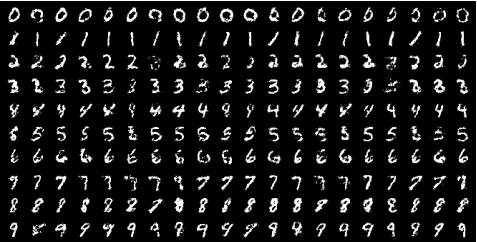
\includegraphics[scale=0.6]{chapter_14/files/conditionalgan.png}
  \caption{ConditionalGAN: Each row of images is generated conditioned on a different class label, leading to different subsets of generated images corresponding to different digits. Images from \cite{mirza2014conditional}}
\end{figure}

\subsection{CycleGAN}
This paper \cite{zhu2017unpaired} proposes a framework for training two generators and two discriminators for translation between two different unpaired image domains, such that the discriminators can't tell the difference between images from domain $Y$ and images generated from domain $X$ that look like domain $Y$, and vice versa. Additionally, a cycle constraint is introduced that minimizes the reconstruction error of translating an image from one domain to the other and back.
\begin{figure}[h]
\centering
  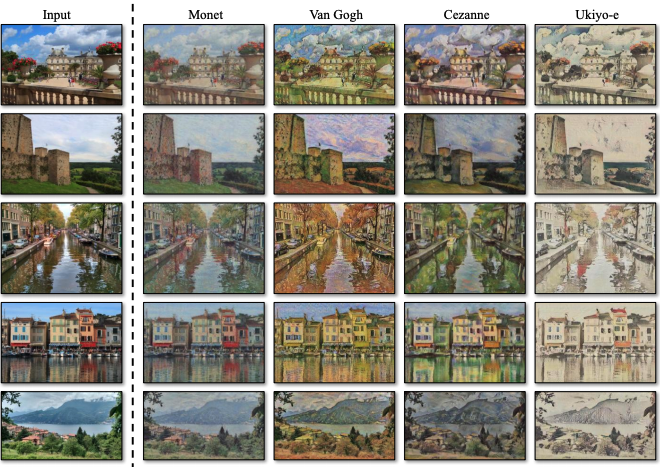
\includegraphics[scale=0.25]{chapter_14/files/cyclegan_art.png}
  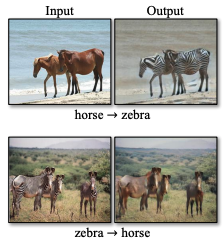
\includegraphics[scale=0.5]{chapter_14/files/cyclegan_horse.png}
  \caption{CycleGAN: Original images and their translated equivalents. Images from \cite{zhu2017unpaired}}
\end{figure}

\subsection{InfoGAN}
This GAN variant \cite{chen2016infogan} adds an additional input $c$ to the generator, then adds an additional loss term to maximise mutual information between the given code $c$ and the images generated from it $G(z;c)$. As such, this encourages learning disentangled latent codes where each feature in $c$ corresponds to some interpretable feaure in the output, like rotations, hair styles, and other visual features in an output image. As such, by varying a single element in the latent code, images can be generated that smoothly vary high-level features in the output.

\subsection{Progressive GAN}
Under the Progreessive GAN framework \cite{karras2017progressive}, both the discriminator and generator are grown from low resolution to high resolution as training progresses by adding more layers to the previously trained lower resolution layers, which both speeds up training and leads to higher quality output.

\subsection{StyleGAN}
StyleGAN \cite{karras2018stylebased} proposes a novel type of generator conditioned on a latent code that is able to separate high level image features from lower level image structure, allowing for the high level appearance of one image to be applied to some other image (a typical style transfer task).

\begin{figure}[h]
\centering
  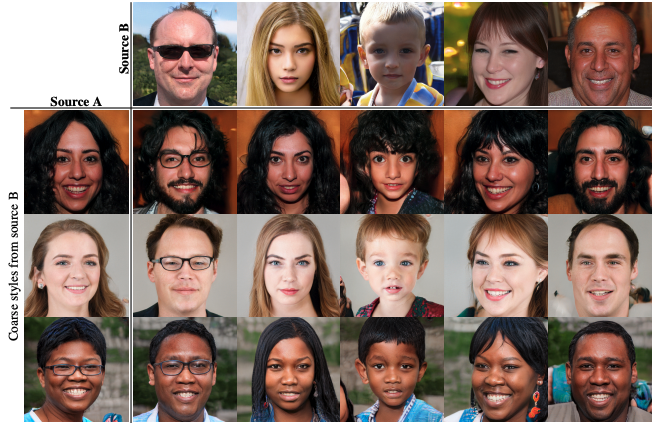
\includegraphics[scale=0.5]{chapter_14/files/stylegan.png}
  \caption{StyleGAN: Generated images using the combined latent codes of the row and column images. Images from \cite{karras2018stylebased}}
\end{figure}